\section{Άσκηση 2}
\subsection{Θεωρητική Ανάλυση}
Γνωρίζουμε ότι ως προς την ταχύτητα του άξονα περιστροφής του ο κινητήρας είναι ένα ευσταθές σύστημα, διότι η ταχύτητα με την πάροδο του χρόνου παίρνει μια συγκεκριμένη τιμή. Αντίθετα, όμως, η θέση του άξονα μεταβάλλεται συνέχεια και, επομένως, ως προς τη θέση του άξονα το σύστημα είναι ασταθές. Σκοπός αυτής της άσκησης, είναι να καταστήσουμε το σύστημα ευσταθές και ως προς την θέση, χρησιμοποιώντας γραμμική ανάδραση καταστάσεων.

Οπως αναφέραμε προηγουμένως, επιλέγουμε μεταβλητές κατάστασης την ταχύτητα $ω$ και την θέση $θ$ του κινητήρα. Ως έξοδο του συστήματος επιλέγουμε την θέση, άρα \(y=θ\). Επομένως, με $x_1 = ω$ και \(x_2 = θ\), έχουμε από το δομικό διάγραμμα:
\begin{align*}
	X_1 &= \frac{k_m}{T_ms+1}U \Rightarrow X_1T_ms + X_1 = k_mU \Rightarrow \dot{x}_1 = -\frac{1}{Tm}x_1 + \frac{k_m}{T_m}u \\
	X_2 &= k_μ\frac{k_0}{s}X_1 \Rightarrow X_2s = k_μk_0X_1 \Rightarrow \dot{x}_2 = k_μk_0x_1 \\
	y &= x_2
\end{align*}
Δηλαδή, αν $x = \begin{bmatrix} x_1 \\ x_2\end{bmatrix}$ το δίανυσμα κατάστασης, το σύστημά μας είναι το \[\dot{x} = Ax + Bu, \quad y = Cx + Du\]
Όπου
\begin{align*}
	A &= \begin{bmatrix} -\frac{1}{T_m} & 0 \\ k_μk_0 & 0\end{bmatrix} \\
	B &= \begin{bmatrix} \frac{k_m}{T_m} \\ 0 \end{bmatrix} \\
	C &= \begin{bmatrix} 0 & 1\end{bmatrix} \\
	D &= \begin{bmatrix} 0 \end{bmatrix}
\end{align*}
Υπολογίζουμε τώρα τον πίνακα ελεγξιμότητας
\[
M = \begin{bmatrix} B & AB \end{bmatrix}
= \renewcommand{\arraystretch}{2.5}
\begin{bmatrix}
\dfrac{k_m}{T_m} & -\dfrac{k_m}{T_m^2} \\
0 & \dfrac{k_\mu k_0 k_m}{T_m}
\end{bmatrix}
\renewcommand{\arraystretch}{1}
\]
Και επειδή \(det(M) = \dfrac{k_m^2k_μk_0}{T_m^2} = 1132.69 \neq 0\), το σύστημά μας είναι ελέγξιμο. Έτσι, μπορούμε να επιλέγξουμε ελεγκτη \(u = -kx + k_rr\), όπου \(k = \begin{bmatrix} k_1 \\ k_2\end{bmatrix}\). Ο όρος \(-kx\) θα μας βοηθήσει ώστε η απόκριση του συστήματος
κλειστού βρόχου να μην παρουσιάζει υπερύψωση και ο χρόνος αποκατάστασης να είναι ο μικρότερος δυνατός, ενώ ο όρος $+k_rr$ θα μας βοηθήσει ώστε η θέση του κινητήρα να συγκλίνει σε μία συγκεκριμένη επιθυμητή τιμή.

Θεωρούμε ότι στην μόνιμη κατάσταση ισχύει $\dot{x} = 0$ και απο θεωρία έχουμε
\[
	k_r = \frac{1}{Dk(A-Bk)^{-1}B+D-C(A-Bk)^{-1}B} \overset{\dots}{=} k_2
\]
Αντικαθιστώντας τον ελεγκτή μας $u=-kx+k_2r$ στο αρχικό μας σύστημα, παίρνουμε το σύστημα
\[
\dot{x} =
\underbrace{
\begin{bmatrix}
  -\frac{1 + k_m k_1}{T_m} & -\frac{k_m k_2}{T_m} \\
  k_μ k_0 & 0
\end{bmatrix}
}_{\tilde{A}} x
+ 
\begin{bmatrix}
  \frac{k_2 k_m}{T_m} \\
  0
\end{bmatrix} r
\]
Με χαρακτηριστικό πολυώνυμο
\[
	P(s) = det(sI - \tilde{A}) = s^2 + \frac{1+k_mk_1}{T_m}s + \frac{k_mk_2k_μk_0}{T_m} = s^2 + 2ζω_ns + ω_n^2
\]
Θέλουμε το σύστημα να είναι ευσταθές, άρα απο κριτήριο Routh-Hurwitz πρέπει
\[
\renewcommand{\arraystretch}{2.5}
\left.
\begin{array}{l}
	\frac{1 + k_m k_1}{T_m} > 0 \\ 
	\frac{k_m k_2 k_μ k_0}{T_m} > 0
\end{array}
\right\}
\Rightarrow
\left.
\begin{array}{l}
	k_1 > -\frac{1}{k_m} = -\frac{1}{218.89} = -4.57 \cdot 10^{-3} \\
	k_2 > 0
\end{array}
\right\}
\renewcommand{\arraystretch}{1}
\]
Επίσης, θέλουμε το σύστημα να μην έχει υπερύψωση, δηλαδη $ζ \geq 1$. Θέλουμε, όμως, και ο χρόνος αποκατάστασης να είναι ο μικρότερος δυνατός, οπότε πρέπει
\begin{equation}
	ζ = 1 \Rightarrow \frac{1+k_mk_1}{2\sqrt{T_mk_mk_2k_μk_0}} = 1 \Rightarrow 1+218.89k_1 = 1.47\sqrt{k_2}
	\label{eq:z}
\end{equation}
\subsection{Εργαστηριακά Αποτελέσματα}
Βάση των παραπάνω περιορισμών, επιλέγουμε $k_1=0.01$ και τότε από την \Cref{eq:z} έχουμε $k_2=4.706$.

\subsubsection{Ερώτημα 1}
Σημαντικό είναι να σημειώσουμε, ότι λόγω προβλήματος στον συγκεκριμένο κινητήρα τον οποίο μελετάμε, για τάση αναφοράς επιλέχθηκε η $θ_{ref} = 8V$ και ως αρχική θέση του κινητήρα η $θ_0=5V$. Έτσι, έχουμε τα παρακάτω αποτελέσματα. Στο διάγραμμα της θέσης «position» μπορούμε να δούμε ότι το σύστημά μας συγκλίνει στην επιθυμητή $θ_{ref} = 8V$ χωρίς ταλαντώσεις και με καλό χρόνο αποκατάστασης.

\begin{figure}[H]
    \centering
    \begin{minipage}{0.45\textwidth}
        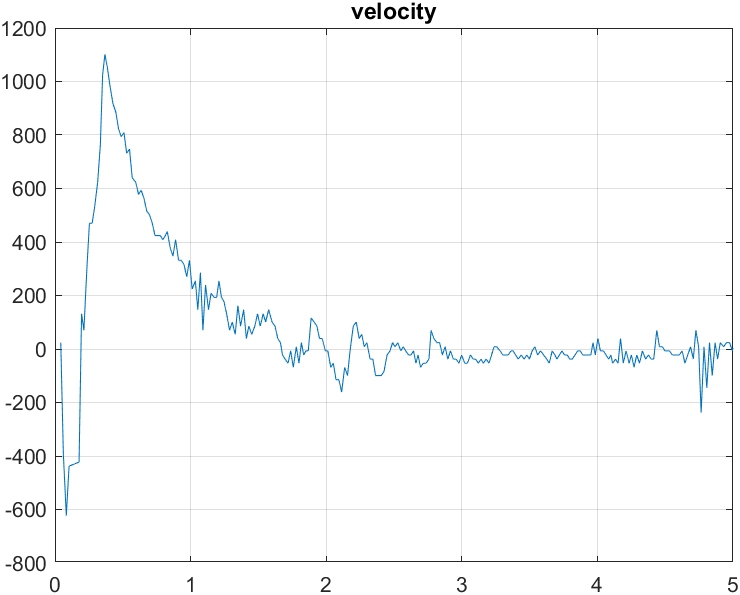
\includegraphics[width=\linewidth]{Images/lab2/1/vel221.png}
    \end{minipage}
    \hfill
    \begin{minipage}{0.45\textwidth}
        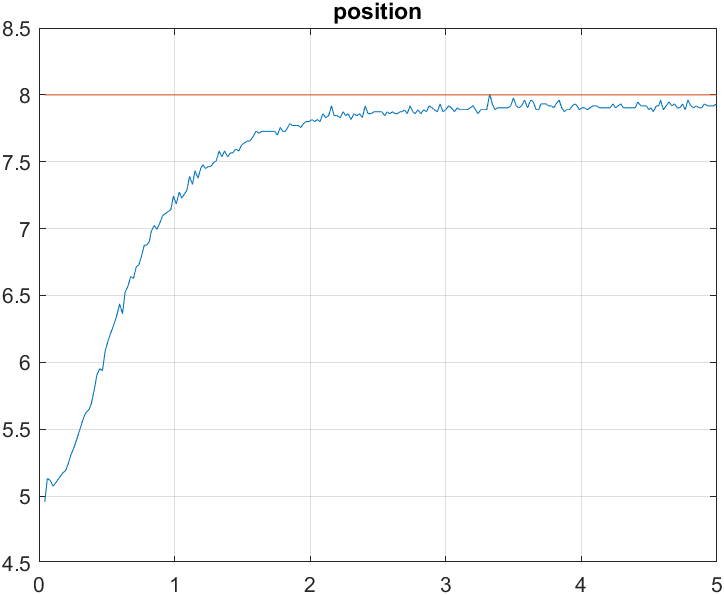
\includegraphics[width=\linewidth]{Images/lab2/1/pos221.png}
    \end{minipage}
    
    \vspace{0.5cm}
    
    \begin{minipage}{0.45\textwidth}
        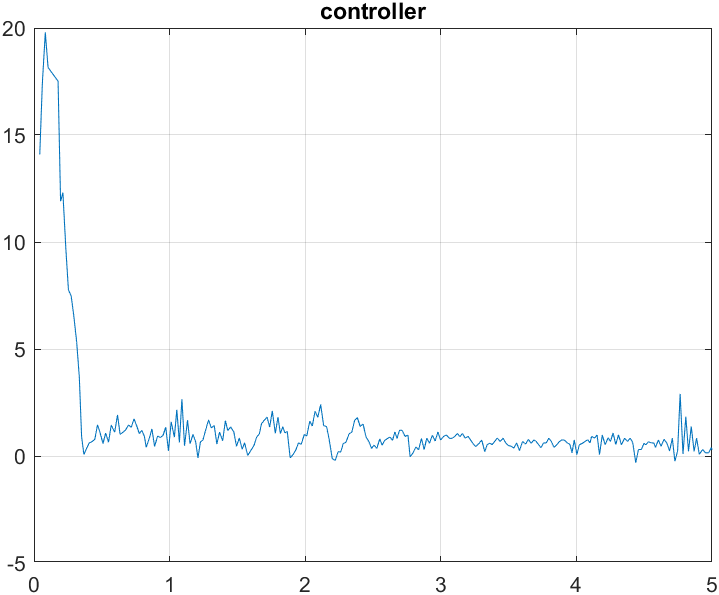
\includegraphics[width=\linewidth]{Images/lab2/1/con221.png}
    \end{minipage}
    \hfill
    \begin{minipage}{0.45\textwidth}
        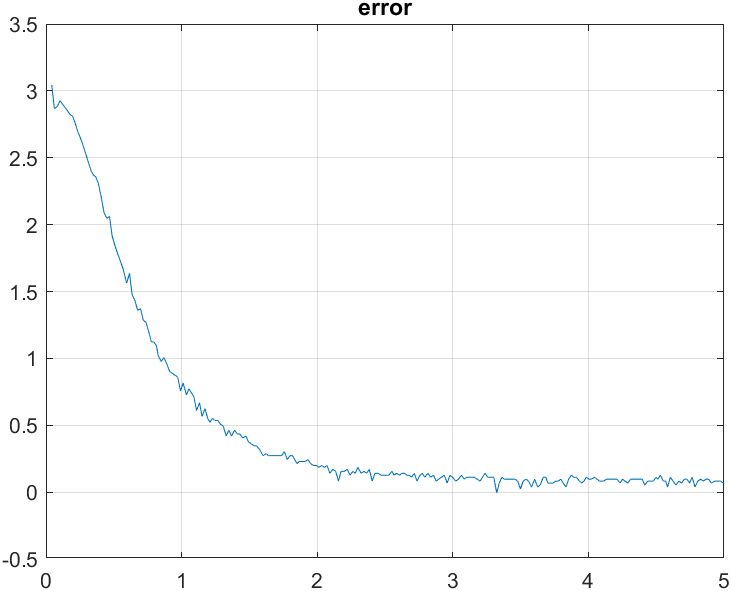
\includegraphics[width=\linewidth]{Images/lab2/1/err221.png}
    \end{minipage}
\end{figure}

\subsubsection{Ερώτημα 2}
Είναι γεγονός ότι έχουμε σφάλμα στην μόνιμη κατάσταση, αφού δεν φτάνουμε ακριβώς στην επιθυμητή τιμή $θ_{ref} = 8V$. Το σφάλμα αυτό οφέιλειται στις τριβές που υπάρχουν και τις οποίες δεν έχουμε με κανένα τρόπο μοντελοποιήσει στο σύστημά μας. Για να το εξαλέιψουμε, πάντως, θα μπορούσαμε να βάλουμε έναν ολοκληρωτή, ο οποίος όπως γνωρίζουμε καθιστά το σφάλμα θέσης μηδενικό.

\subsubsection{Ερώτημα 3}
Κατεβάζουμε το μαγνητικό φρένο του κινητήρα και επαναλαμβάνουμε τις μετρήσεις μας με τα ίδια κέρδη. Όπως παρατηρουμε στα ακόλουθα διαγράμματα, οι διαφορές είναι ελάχιστες. Ο λόγος είναι ότι το φρένο έχει απομαγνητιστεί, οπότε δεν δημιουργεί κάποια ουσιαστική διαφορά στο σύστημα. Κανονικά θα περιμέναμε να παρατηρήσουμε μια πιο αργή απόκριση. Είναι, πάντως, εμφανής μία μικρή αλλαγή στην ταχύτητα του κινητήρα, αφού χωρίς το φρένο είχε peak τα 1100rpm, ενώ το φρένο κατεβάζει αυτό το νούμερο στα 1000rpm, το οποίο είναι ένα λογικό αποτέλεσμα του φρεναρίσματος.

\begin{figure}[H]
    \centering
    \begin{minipage}{0.45\textwidth}
        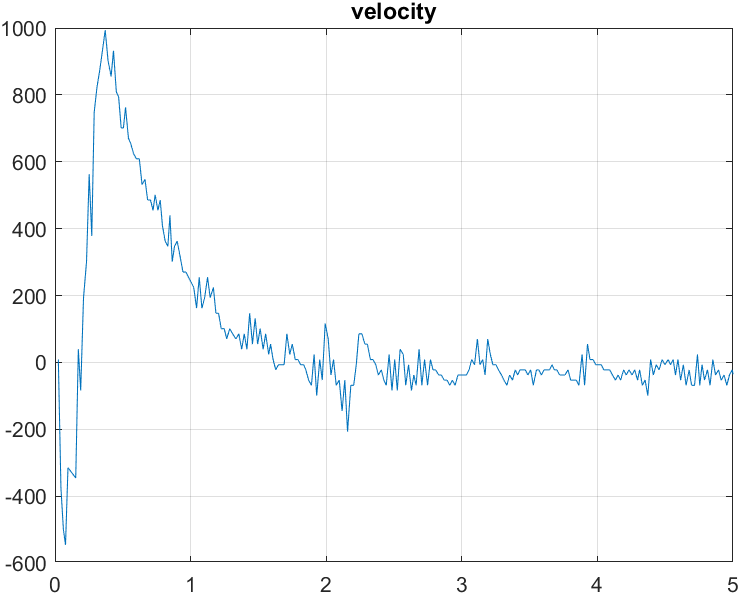
\includegraphics[width=\linewidth]{Images/lab2/3/vel223.png}
    \end{minipage}
    \hfill
    \begin{minipage}{0.45\textwidth}
        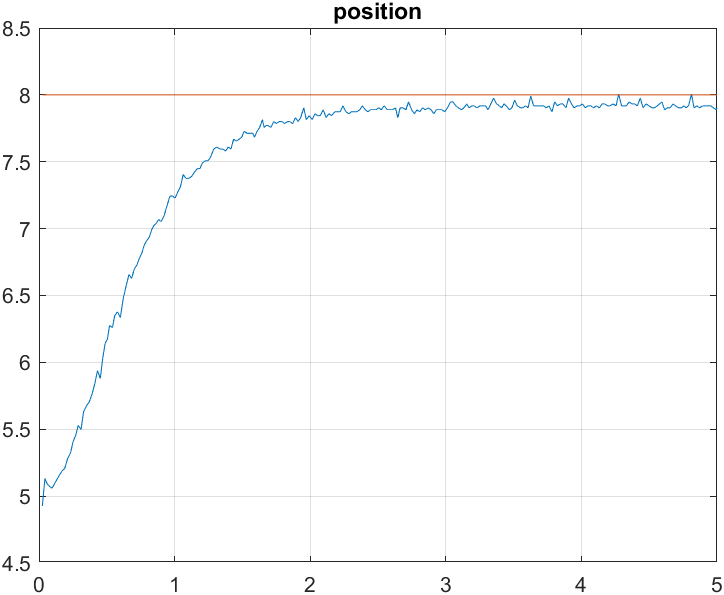
\includegraphics[width=\linewidth]{Images/lab2/3/pos223.png}
    \end{minipage}
    
    \vspace{0.5cm}
    
    \begin{minipage}{0.45\textwidth}
        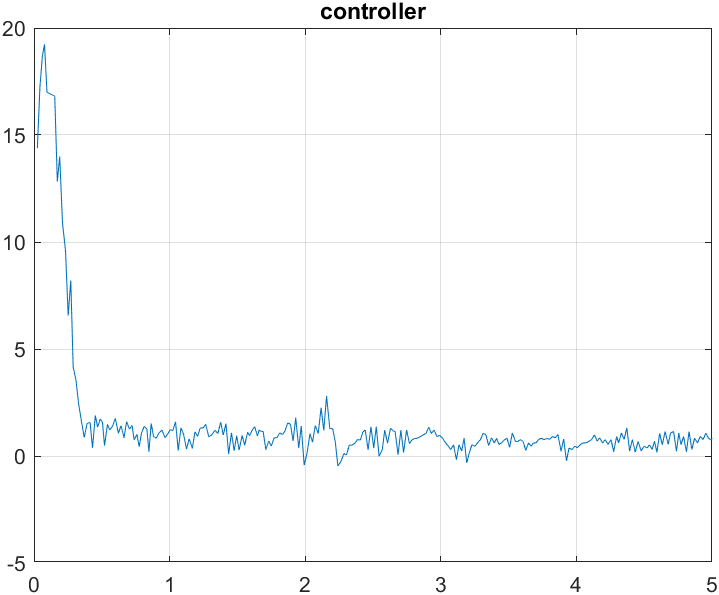
\includegraphics[width=\linewidth]{Images/lab2/3/con223.png}
    \end{minipage}
    \hfill
    \begin{minipage}{0.45\textwidth}
        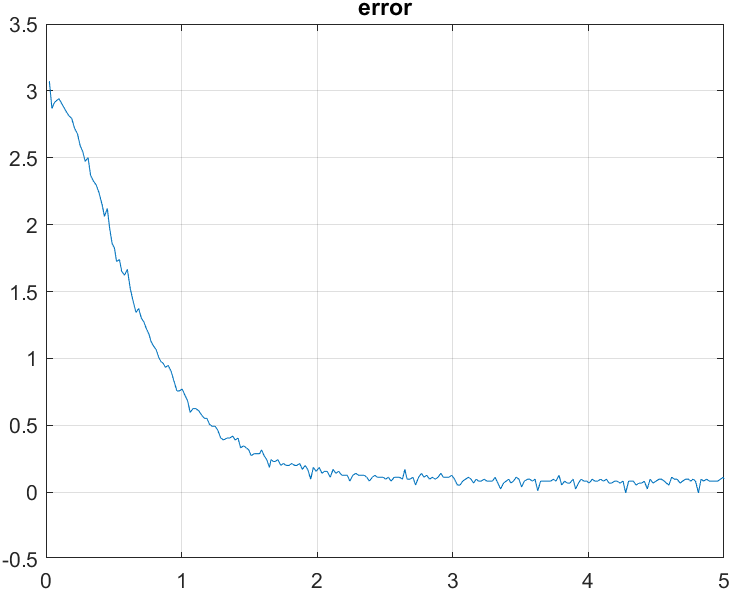
\includegraphics[width=\linewidth]{Images/lab2/3/err223.png}
    \end{minipage}
\end{figure}
\newpage
\subsubsection{Ερώτημα 4}
Ανεβάζουμε το μαγνητικό φρένο και επαναλαμβάνουμε με τα αρχικά μας κέρδη τον έλεγχο, μόνο που πλέον η επιθυμητή μας θέση είναι η $θ_{ref} = 8+2\sin(ωt)$. 
\begin{enumerate}
	\item Για 3 περιόδους σε $5sec$, δηλαδή $ω_1 = \dfrac{6π}{5} rad/s$, έχουμε
\begin{figure}[H]
    \centering
    \begin{minipage}{0.45\textwidth}
        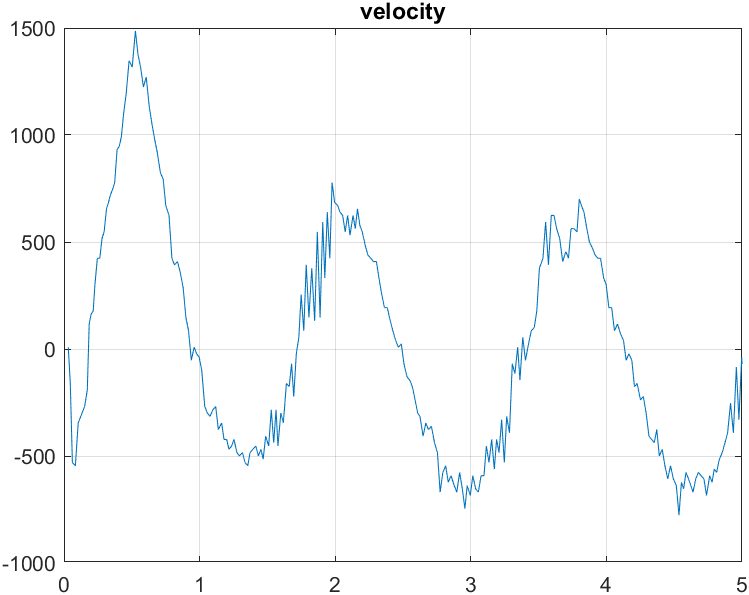
\includegraphics[width=\linewidth]{Images/lab2/4/1/vel2241.png}
    \end{minipage}
    \hfill
    \begin{minipage}{0.45\textwidth}
        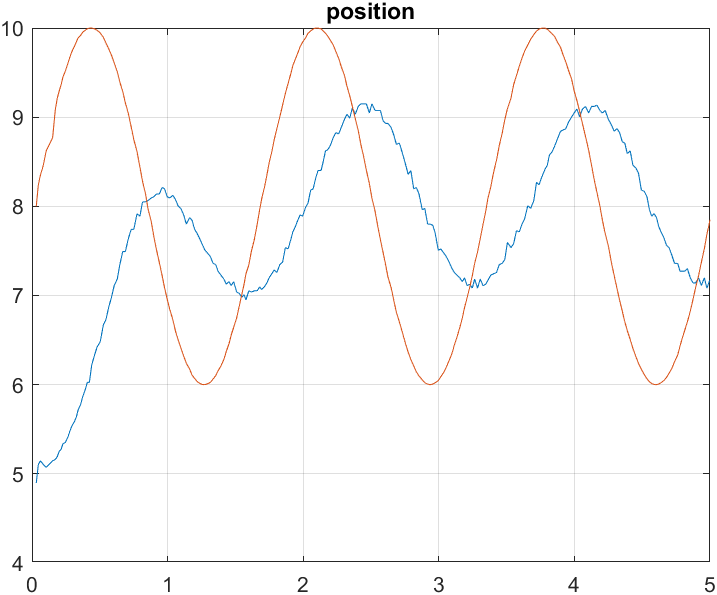
\includegraphics[width=\linewidth]{Images/lab2/4/1/pos2241.png}
    \end{minipage}
    
\end{figure}
\begin{figure}[H]
    \begin{minipage}{0.45\textwidth}
        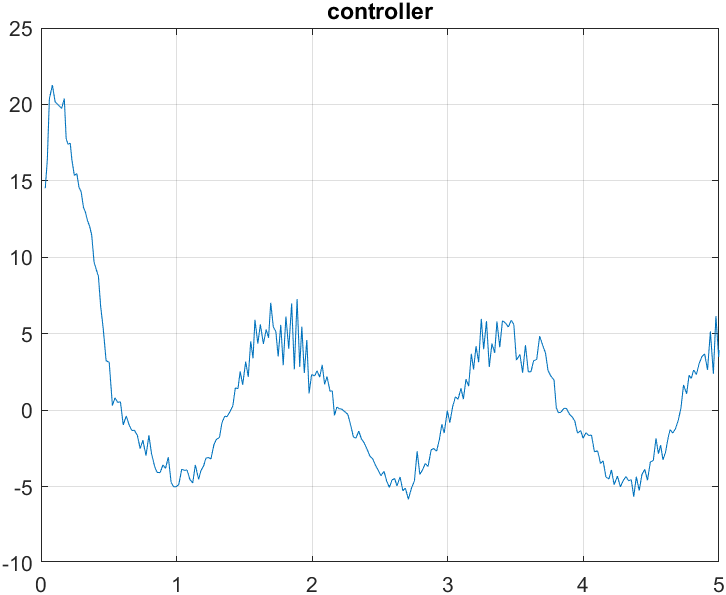
\includegraphics[width=\linewidth]{Images/lab2/4/1/con2241.png}
    \end{minipage}
    \hfill
    \begin{minipage}{0.45\textwidth}
        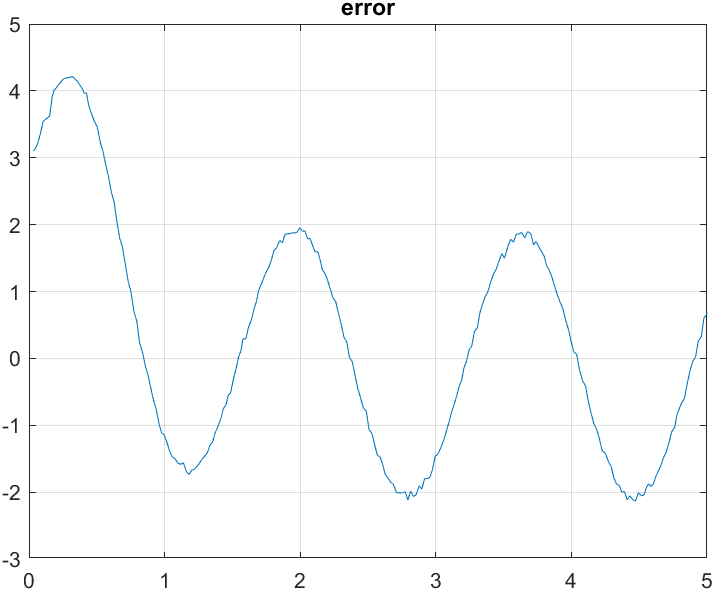
\includegraphics[width=\linewidth]{Images/lab2/4/1/err2241.png}
    \end{minipage}
\end{figure}
	\item Για 1 περίοδο σε $5sec$, δηλαδή $ω_2 = \dfrac{2π}{5} rad/s$, έχουμε

    \begin{figure}[H]
    \centering
    \begin{minipage}{0.45\textwidth}
        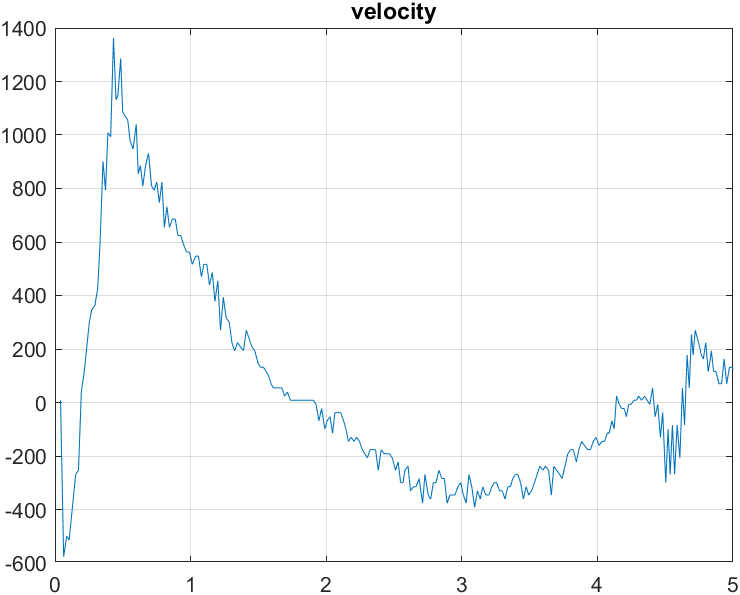
\includegraphics[width=\linewidth]{Images/lab2/4/2/vel2242.png}
    \end{minipage}
    \hfill
    \begin{minipage}{0.45\textwidth}
        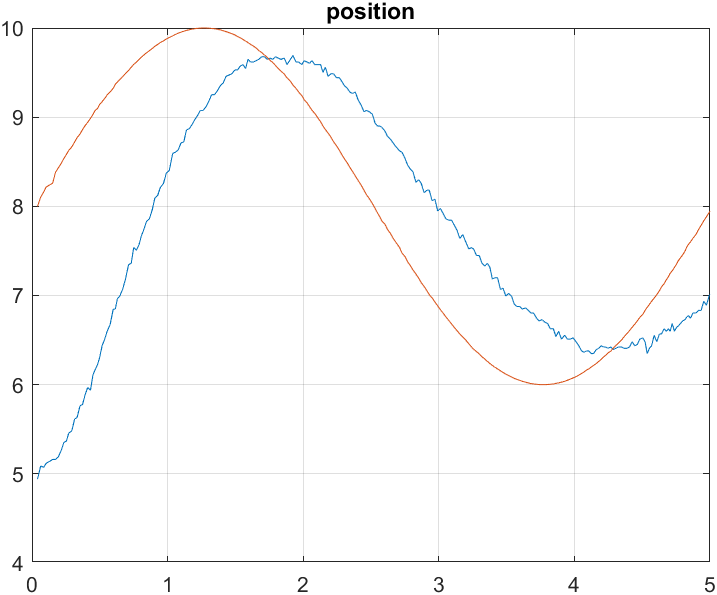
\includegraphics[width=\linewidth]{Images/lab2/4/2/pos2242.png}
    \end{minipage}
    
    \vspace{0.5cm}
    
    \begin{minipage}{0.45\textwidth}
        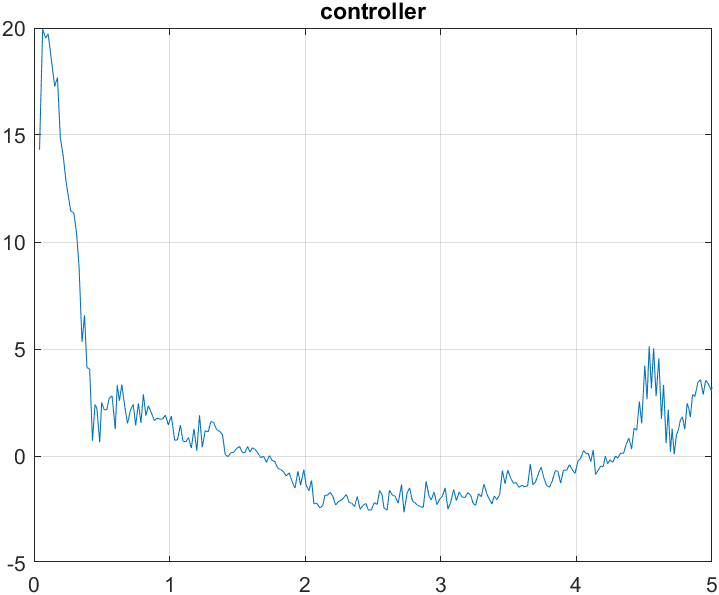
\includegraphics[width=\linewidth]{Images/lab2/4/2/con2242.png}
    \end{minipage}
    \hfill
    \begin{minipage}{0.45\textwidth}
        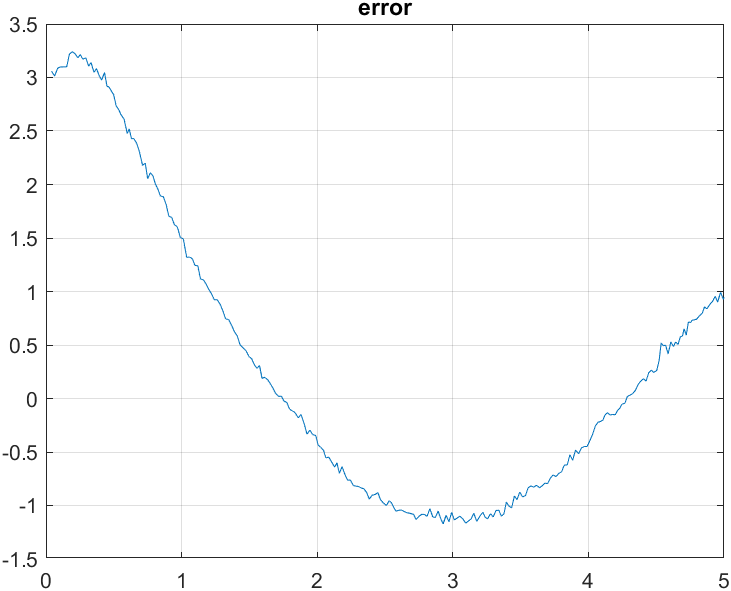
\includegraphics[width=\linewidth]{Images/lab2/4/2/err2242.png}
    \end{minipage}
\end{figure}
	\item Για 1 περίοδο σε $20sec$, δηλαδή $ω_3 = \dfrac{2π}{20} rad/s$, έχουμε
    \begin{figure}[H]
    \centering
    \begin{minipage}{0.44\textwidth}
        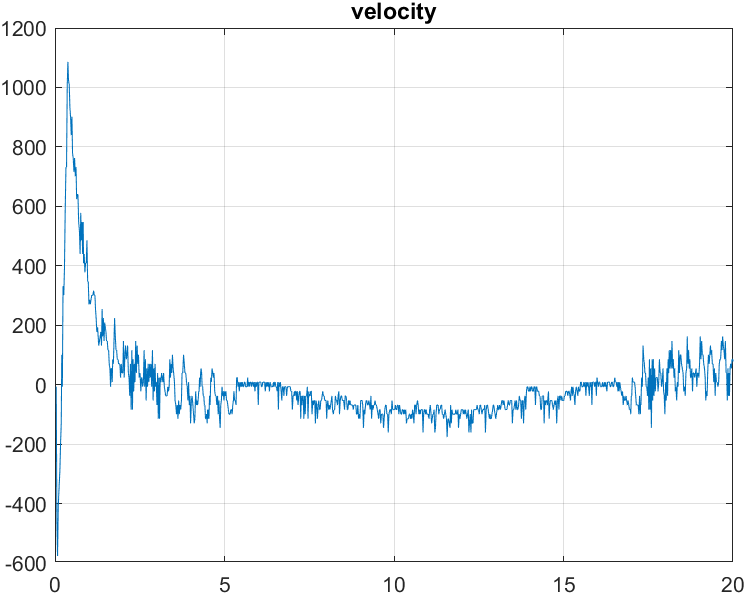
\includegraphics[width=\linewidth]{Images/lab2/4/3/vel2243.png}
    \end{minipage}
    \hfill
    \begin{minipage}{0.44\textwidth}
        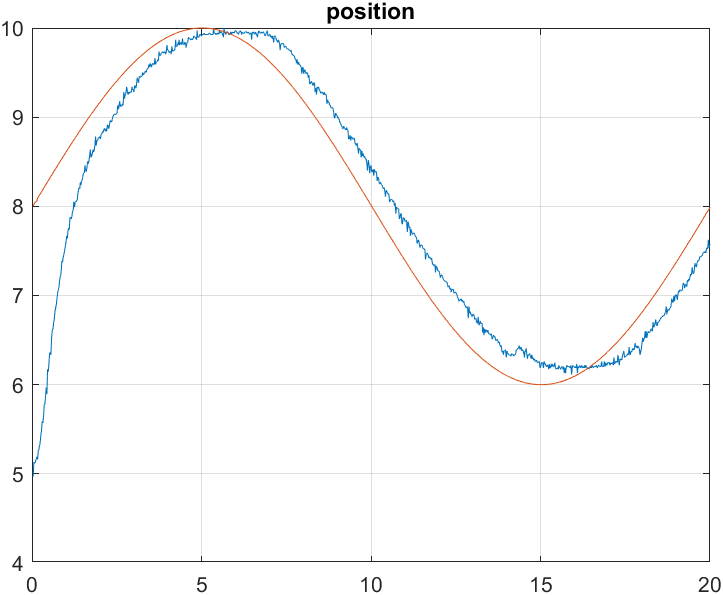
\includegraphics[width=\linewidth]{Images/lab2/4/3/pos2243.png}
    \end{minipage}
    
    \end{figure}
    \begin{figure}[H]
    \begin{minipage}{0.45\textwidth}
        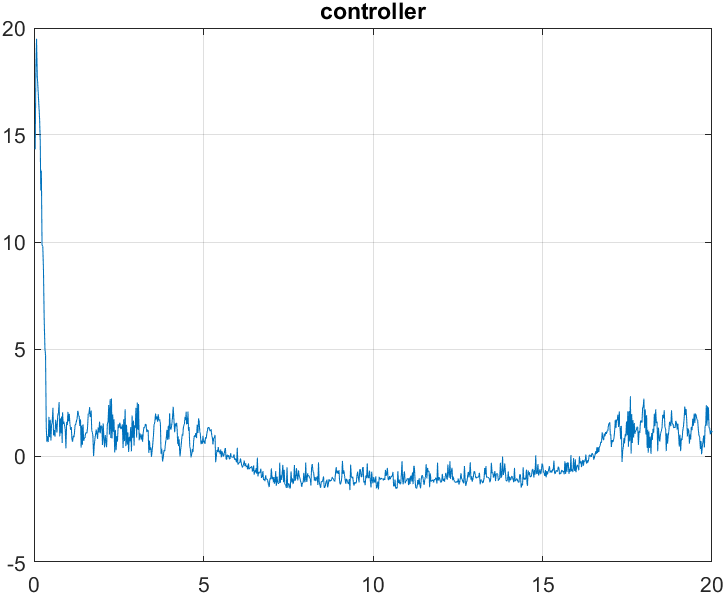
\includegraphics[width=\linewidth]{Images/lab2/4/3/con2243.png}
    \end{minipage}
    \hfill
    \begin{minipage}{0.45\textwidth}
        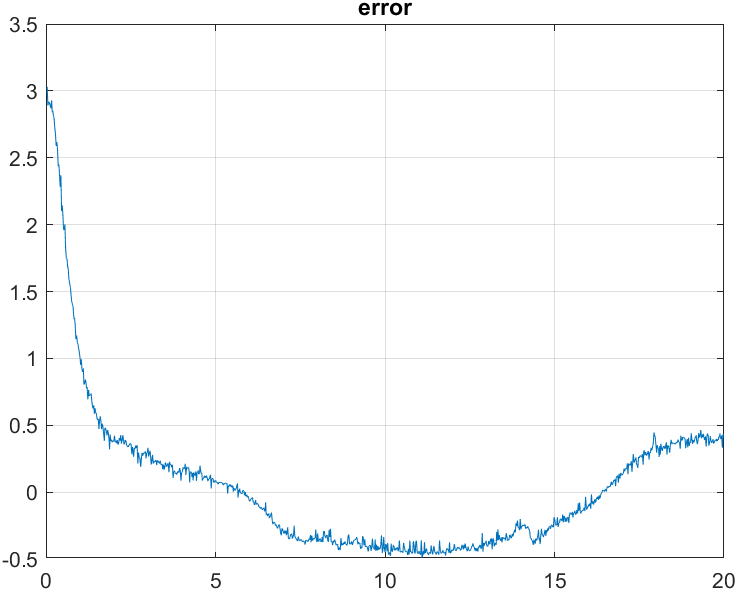
\includegraphics[width=\linewidth]{Images/lab2/4/3/err2243.png}
    \end{minipage}
\end{figure}
\end{enumerate}
Παρατηρούμε ότι τόσο στην $ω_1$, όσο και στην $ω_2$, δηλαδή σε μεσαίες συχνότητες, η απόκριση μεταβάλλεται ημιτονοειδώς με τον χρόνο. Βέβαια, στην μικρότερη εκ των δύο συχνότητα $ω_2 < ω_1$ η έξοδος ακολουθεί πιο καλά την επιθυμητή έξοδο. Όμοια και στην μικρή συχνότητα $ω_3$, η απόκριση προσεγγίζει πολύ καλά την $θ_{ref}$, καλύτερα από τις άλλες δύο μεγαλύτερες συχνότητες.